
\begin{table}
	\caption{Dataset Statistics for CHEMET}
	\centering
	\begin{tabular}{lllll}
		
		\toprule
		Setting &Anno.& \#Inst. & \#Entity  & \#Types \\
		\midrule
		Train &Distant&   1000& NA&39\\
		Dev &Human&500&NA&39\\
		Test&Human&            500&NA&39 \\
		\bottomrule
	\end{tabular}
	\label{datastats}
\end{table}

\begin{figure*}[ht]
% 	\vskip 0.2in
	\begin{center}
		\centerline{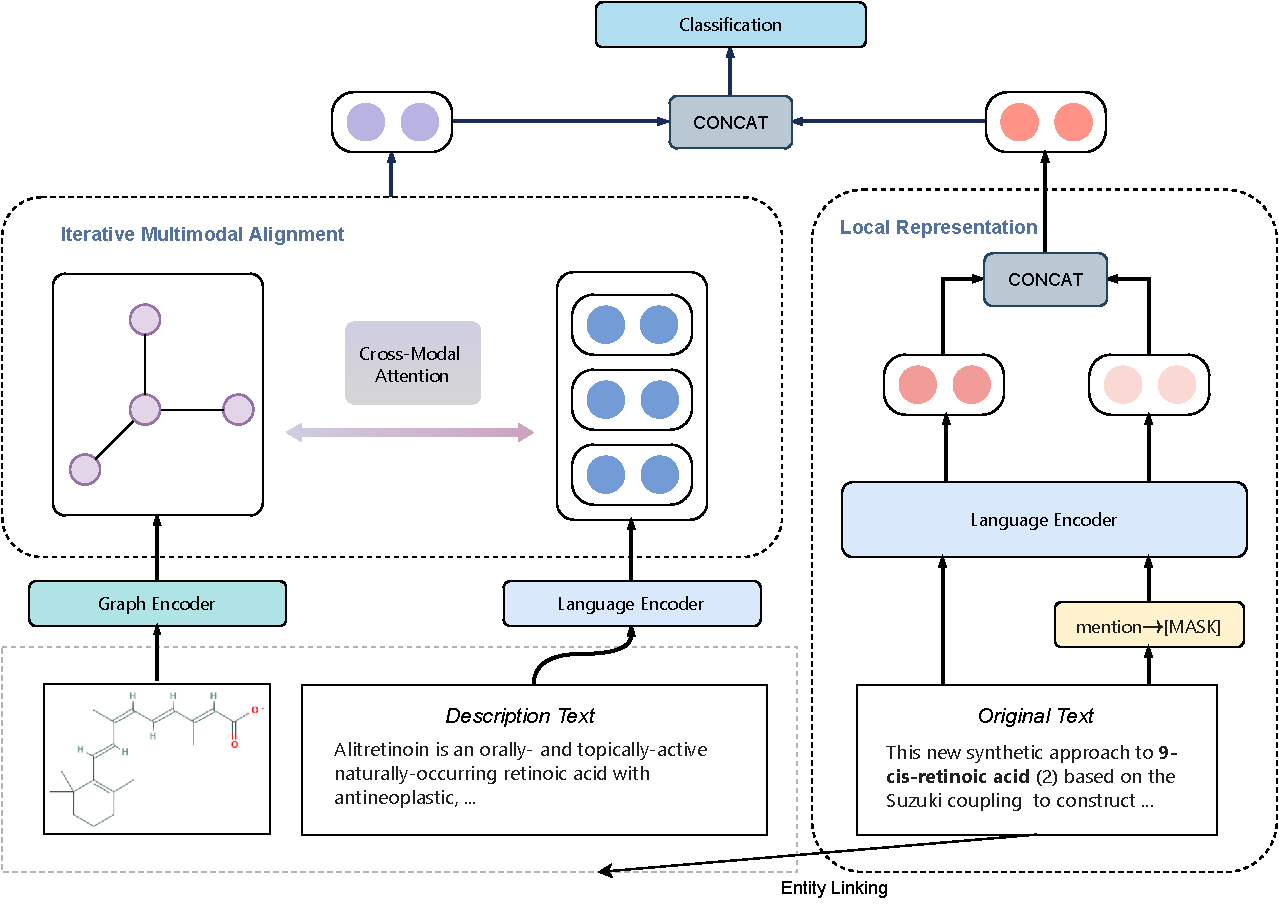
\includegraphics[width=1.8 
			\columnwidth]{model_new.pdf}}
		\caption{Our fine-grained chemical entity typing model architecture. Please refer to Section~\ref{sec:method} for details.}
		\label{fig:framework}
	\end{center}
	\vskip -0.2in
\end{figure*}
\section{Dataset}
%\subsection{Data Collection}
\label{datacollection}

% Krippendorff alpha, or other 
agreement metric

describe diversity

\cheng{"limited dataset" is a bit vague. Is there any such data set available? If so, we should try to use it. My sense is that there isn't(?), so the novelty and significance of the data set could be more clearly articulated.}
Due to limited dataset being available for fined-grained chemical entity typing, we have collected and annotated a dataset, CHEMET, based on a corpus of 50 papers from PubChem\footnote{\url{https://pubchem.ncbi.nlm.nih.gov/}}) with Suzuki-Coupling (a popular reaction mechanism) theme; the theme was chosen to align with chemistry specialists' domain knowledge. We will discuss the steps taken to construct the dataset below.

\noindent \textbf{Taxonomy Construction}. \cheng{how was the number 39 determined? try to give a justification or explanation of the process that reached the number 39. } We carefully select 39 sub-categories from wikipedia chemistry category page~\footnote{\url{https://en.wikipedia.org/wiki/Category:Chemistry}} as fine-grained ontology; for example, Organic chemistry$\rightarrow$Organic compounds$\rightarrow$Esters is a fined-grained type where right of the arrow is the sub-category of the left. \cheng{The following sentence can be moved earlier in this paragraph to explain the strategy being taken. It's better to first give a description of our goal/strategy/philosophy and then describe how we do it. If there are decisions to be made, explain why we've decided to choose one options not another.} We focused on types that are compound types commonly occurring in Suzuki-Coupling literature. The entire ontology is shown in Appendix~\ref{sec:appendix1}.

\noindent \textbf{Distant Supervision} In order to ease human annotators' work and to collect training data, we employed distant supervision to retrieve noisy labels for the corpus. In this step we first tokenized text using~\cite{oscar4}, a texting mining framework for chemistry that recognize complex chemical name well. We then collected a dictionary mapping from picked types (that is, the select categories from Wikipedia) to their belonging wikipedia pages. We treated the page titles as entity names. Since a compound can have many synonyms, we queried PubChem to expand the dictionary. Finally, we used the dictionary to label the tokenized text using a well-performing string matching algorithm. \cheng{Provide a reference to this string matching algorithm or elaborate.}

\noindent \textbf{Human Annotation}. 
We hired five undergraduate chemistry students as annotators. The annotators were instructed to identify and type spans in the assigned samples using Brat~\cite{brat} interface. To ensure the diversity of the testing data, we randomly select the test samples from the corpus for annotation. In order to mitigate annotator bias, we distributed each sentence to three annotators, and take majority vote from the results. The dataset statistics is shown in Table~\ref{datastats}.


%\subsection{Data Analysis}

%\label{dataanalyze}
%\noindent \textbf{Size}. 
%
%\noindent \textbf{Entity Types}. 